\subsection{Если множество $A$ бесконечно, а множество $B$ конечно или счётно, то множество $A \cup B$ равномощно $A$. Равномощность множеств: бесконечных последовательностей из 0 и 1; вещественных чисел; $[0, 1]; [0, 1)$; множества всех подмножеств натуральных чисел. Равномощность отрезка и квадрата.}
\textbf{Если множество $A$ бесконечно, а множество $B$ конечно или счётно, то множество $A \cup B$ равномощно $A$.}\\

Пусть $A$ - бесконечно, $B$ - не более, чем счетное. Тогда $A \cup B \sim A$.\\

\noindent \textbf{Доказательство:} \\

$B' = B \backslash A$, $B'$ - не более, чем счетное. Очевидно, что $A \cup B = A \cup B'$, но $A$ и $B'$ - не пересекаются.
Так как $A$ - бесконечно, то $\exists C \subseteq A, C$ - счетно. Так как $C \cup B'$ - счетно, то $C \sim C \cup B'$. Значит
$\exists f : C \to C \cup B'$ - биекция.

\begin{figure}[H]
\centering
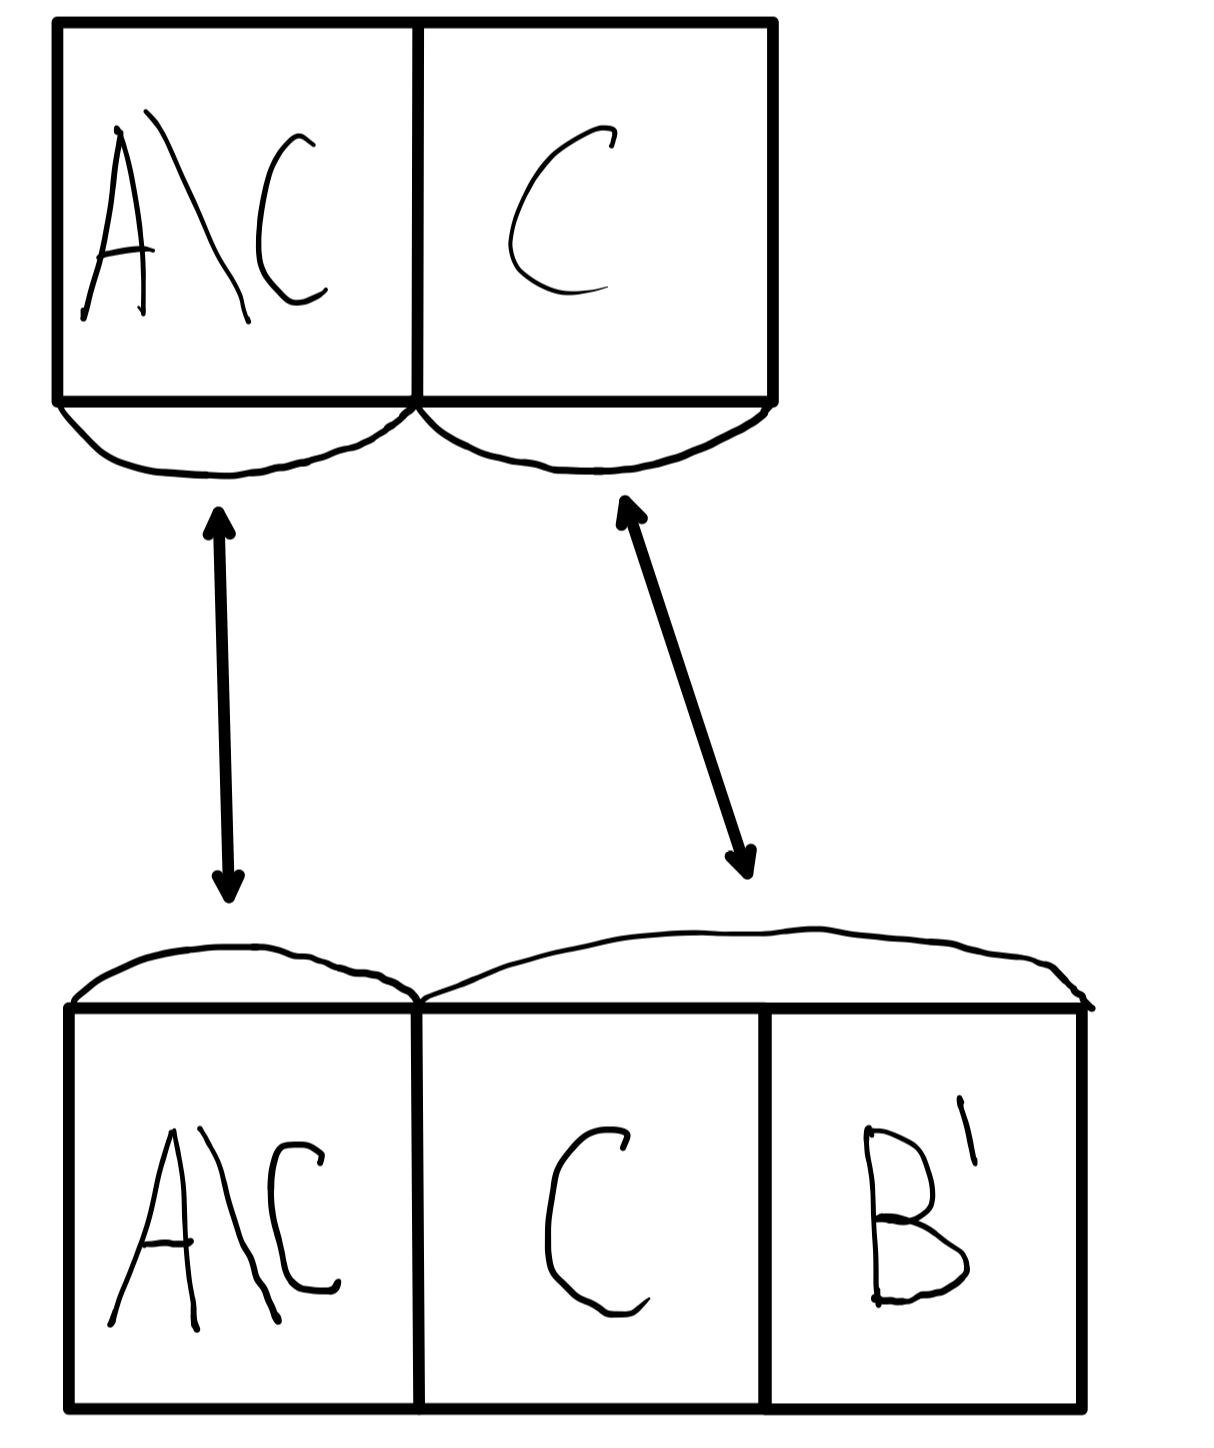
\includegraphics[width=0.3\linewidth]{proofs/images/question16.png}
\caption{иллюстрация биекции}
\end{figure}

Теперь просто построим биекцию $g : A \to A \cup B'$.

\begin{equation*}
    g(a) = \begin{cases}
        f(a), \text{если } a \in C\\
        a, \text{иначе}
    \end{cases}
\end{equation*}

\textbf{Равномощность множеств: $\mathbb{B}^{\infty} \sim [0, 1) \sim [0,1] \sim \R \sim 2^{\N}$.}\\

\noindent \textbf{Доказательство $\mathbb{B}^{\infty} \sim [0, 1)$:} \\

Построим биекцию $f : \mathbb{B}^{\infty} \to [0, 1)$. Инициализируем f(b) так:

Пусть $b = b_0 b_1 b_2 ...$, тогда разделим полуинтервал напополам, если $b_0 = 0$, то перейдем в левую половину и запустимся рекурсивно,
если $b_0 = 1$, то вправо. Так мы сможем получить любые числа на полуинтервале $[0, 1)$, но это не будет биекцией, так как некоторые числа
можно получить двумя способами. К примеру, $\frac{1}{2}$ будет соответствовать последовательность $01111...$ и $10000...$. Поэтому давайте просто
запретим последовательности, которые заканчиваются на бесконечную последовательность 1. Тогда $\mathbb{B}^{\infty} = \mathbb{B}' \cup Y$, где
$Y = \{(*******0), 1111...\}$ - все последовательности, которые заканчиваются на все 1. Но $Y = \bigcup\limits_{k = 0}^{\infty} Y_k$,
где $Y_k = \{a_1, a_2, ..., a_{k - 1}, 0, 1, 1, 1, ...\}$, но $Y_k$ - конечно($|Y_k| = 2^{k-1}$). Значит $Y$ - счетно, а $\mathbb{B}' \sim [0, 1)$, так
как мы исключили плохие случаи, то верно, что

\begin{equation*}
    \mathbb{B}^{\infty} = \mathbb{B}' \cup Y \sim \mathbb{B}' \sim [0, 1)
\end{equation*}

\noindent \textbf{Доказательство $[0, 1) \sim [0, 1] \sim \R$:} \\

Добавление конечного не меняет мощность, поэтому $[0, 1) \sim [0, 1] \sim (0, 1)$. Заметим, что $(0, 1) \sim (-\frac{\pi}{2}, \frac{\pi}{2})$, тут
легко строится биекция $f : (0, 1) \to (-\frac{\pi}{2}, \frac{\pi}{2})$, $f(x) = x \cdot \pi - \frac{\pi}{2}$. Пусть $g : (-\frac{\pi}{2}, \frac{\pi}{2})
\to \R$ и $g(x) = \tg x$ - это очевидно биекция, тогда $(-\frac{\pi}{2}, \frac{\pi}{2}) \sim \R$. Значит $[0, 1) \sim [0, 1] \sim (0, 1) \sim (-\frac{\pi}{2}, \frac{\pi}{2}) \sim \R$.\\

\noindent \textbf{Доказательство $\mathbb{B}^{\infty} \sim 2^{\N}$:}\\

Тут довольно легко построить биекцию. Пусть дана двоичная последовательность $b = b_1 b_2 b_3 ...$. Тогда если $b_i = 1$, то мы берем число $i$ в наше
подмножество, а если $0$, то не берем. При таком кодировании очевидно все подмножества будут различны. Аналогично можно восстановить бинарную
последовательность из данного подмножества.\\

\textbf{Равномощность отрезка и квадрата.}\\

Было доказано, что $\mathbb{B}^{\infty} \to [0, 1]$. Докажем, что $\mathbb{B}^{\infty} \to \mathbb{B}^{\infty} \times \mathbb{B}^{\infty}$.
Построим биекцию $f : (\mathbb{B}^{\infty})^2 \to \mathbb{B}^{\infty}$, наглядно продемонстрируем работу $f((a, b))$

\begin{equation*}
\begin{matrix}
    a_1 a_2 a_3 a_4 ...\\
    b_1 b_2 b_3 b_4 ...
\end{matrix} \Bigg\}
\xrightarrow{\mbox{f}} a_1 b_1 a_2 b_2 a_3 b_3 ...
\end{equation*}

Значит $[0, 1] \sim \mathbb{B}^{\infty} \sim (\mathbb{B}^{\infty} )^2 \sim [0, 1]^2$.